
\subsection{Konstrukcja silnika}\label{sub:konstrukcja silnika}
\paragraph{}

Silnik jest silnikiem wielo-przejściowym. Dla wyświetlenia planet wraz z oświetleniem i teksturami, potrzebne są trzy przejścia. Jedno do wygenerowania g-bufora, oraz dwa do wygenerowania końcowego obrazu. Ponieważ w tym podejściu niemożliwe jest uzyskani przezroczystości, aby wyświetlić półprzezroczyste atmosfery konieczne jest wyświetlenie ich oddzielnie. Są one podobnie jak planety wyświetlanie kolejnymi dwoma przejściami przy użyciu deferred renderingu. Cały silnik posiada więc pięć przejść, trzy dla obrazów planet i dwa dla atmosfer. Następnie wyniki tych przejść są nakładane na siebie z uwzględnieniem przezroczystości atmosfer.

\subsection{Dane pośrednie}\label{sub:dane pośrednie}
\paragraph{}

Silnik graficzny potrzebuje dużego bufora pośrednich danych. Buforem tym z uwagi na wygodę używania jest dwuwymiarowa tekstura zmiennoprzecinkowa. Jednostka renderująca jest w stanie zapisać wartość do jednego teksela tekstury na której pracuje. Największy teksel jaki jest obsługiwany zawiera cztery zmiennoprzecinkowe liczby typu float. Ponieważ do wyrednerowania końcowego obrazu potrzebne jest 16 floatów danych dla każdego piksela, konieczne jest użycie czterech tekstur pośrednich. Z tego powodu metoda ta jest ograniczona jedynie dla nowych kart graficznych posiadających technologię MTR (Multiple Target Render). Dane zawarte w buforach pośrednich przedstawiają się następująco:

\begin{verbatim}
 buffers   |          values 
-----------+--------+--------+--------+----------
 texture 1 | pos.x  | pos.y  | pos.z  | alpha
 texture 2 | norm.x | norm.y | norm.z | acol.r
 texture 3 | col.r  | col.g  | col.b  | acol.g   
 texture 4 | ke     | ka     | kd     | acol.b
\end{verbatim}

Znaczenie poszczególnych danych przedstawione jest poniżej:

\begin{description}
\item[pos] -- trójelementowy wektor oznaczający pozycję powierzchni w danym pikselu
\item[norm] -- wektor normalny powierzchni w danym pikselu
\item[col] -- kolor bazowy danego piksela (bez oświetlenia, po nałożeniu tekstury)
\item[alpha] -- przezroczystość planety. Przyjmuje wartości 1.0 dla koła oznaczającego planetę i 0.0 dla braku planety. Umieszczony jest oddzielnie od koloru, ponieważ geometry shader potrzebuje zarówno pozycji, jak i wartości przezroczystości, a dzięki takiemu układowi danych może on próbkować tylko jedną teksturę.
\item[acol] -- kolor atmosfery otaczającej planetę. Jest trzymany oddzielnie, ponieważ na atmosferę trochę inaczej działa oświetlenie.
\item[ke] -- współczynnik materiału dla światła emitowanego. Jeśli jest większy od zera, planeta będzie źródłem światła.
\item[ka] -- współczynnik materiału dla światła otoczenia (ambient). Działa podobnie co emitowane, jednak nie sprawia że planeta staje się sama źródłem światła dla innych.
\item[kd] -- współczynnik materiału dla światła rozproszonego (diffuse). Standardowy współczynnik z modelu oświetlenia Phonga.
\end{description}

\paragraph{}

Taka wielkość bufora geometrii może sprawiać wrażenie bardzo dużej. Jednak przy przepustowościach nowoczesnych kart jest to w zupełności akceptowalna wielkość. Łatwo można policzyć teoretyczną wartość fps (klatek/sek), gdyby program zajmował się jedynie wypełnianiem g-bufora. Bufory dla rozdzielczości fullhd, czyli 1920$\times$1080 pikseli zajmują około $32MB$. Przepustowość karty graficznej, na której były prowadzone testy (geforce 9800GTX), wynosi 70GB/s. Teoretyczna maksymalna wartość fps wynosi więc:

$$ Buffor size = 1920 \cdot 1080 \cdot 4 \cdot 4B \simeq 32MB $$
$$ \frac{Bandwidth}{Buffor size} = \frac{70GB/s}{32MB} = 2240 fps $$

Jest to więc wielkość całkiem spora, ponieważ aby program dalej móc nazywać programem czasu rzeczywistego, mógłby on wypełniać 100 takich buforów w każdej klatce programu.

\paragraph{}

Również w specyfikacji OpenGLa w wersji 3.2, do którego się ograniczyliśmy,  jest napisane że minimalna ilość jednostek docelowych do których może wyświetlać dane potok, musi wynosić 8 lub więcej. Oznacza to więc, że każda karta graficzna spełniająca wymagania będzie w stanie wydajnie obsługiwać tak duże bufory ramki.


\subsection{Generowanie geometrii}\label{sub:generowanie geometrii}
\paragraph{}

Pierwsze podejście do silnika graficznego opierało się na zwykłym podejściu forward renderingu, z wykorzystaniem geometry shaderów. Jednak kula która daje zadowalający efekt i jest wyświetlana przy pomocy zestawu wierzchołków, musiała by ich mieć około tysiąca. Samo przetwarzanie takiej geometrii jest kosztowne, dodatkowo doszły do tego ograniczenia karty graficznej i geometry shaderów. Pierwsze podejścia do generowania geometrii zakładały generowanie chmury cząstek wokół punktu reprezentującego pozycję planety. Jednak jednym geometry shaderem można było wygenerować jedynie około stu wierzchołków. Kolejne podejścia polegające na "zlepianiu" kul z kilku przejść geometry shadera, okazały się być skrajnie niewydajne. Z pomocą przyszedł lekko zmodyfikowany deferred rendering, który pozwala dla każdej planety generować jedynie cztery wierzchołki. Na rysunku \hyperref[fig:geom]{\ref*{fig:geom}} porównane są wyniki 'sklejanych' kul z końcowym efektem. Co prawda ilość wierzchołków w trzech pierwszych modelach można zmniejszyć trzykrotnie używając łańcucha trójkątów, to nawet trzykrotny wzrost wydajności nie wystarczył by, aby ta technika mogła być użyta.

\begin{figure}
\centering
\label{fig:geom}
	\subfloat[60]   {\label{fig:sph0}   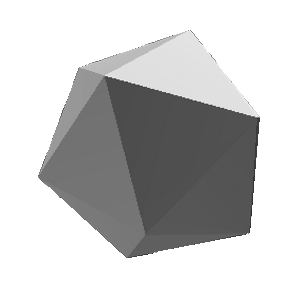
\includegraphics[width=0.25\textwidth]{img/sph_0.png}}   \hspace{.0\textwidth}
	\subfloat[960]  {\label{fig:sph2}   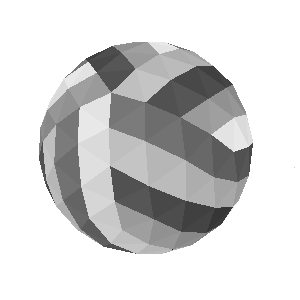
\includegraphics[width=0.25\textwidth]{img/sph_2.png}}   \hspace{.0\textwidth}
	\subfloat[61440]{\label{fig:sph5}   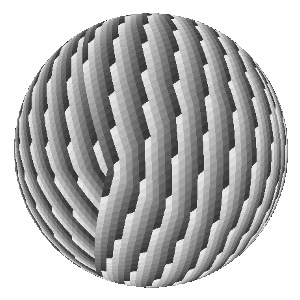
\includegraphics[width=0.25\textwidth]{img/sph_5.png}}   \hspace{.0\textwidth} \\
	\subfloat[4]    {\label{fig:sph_def}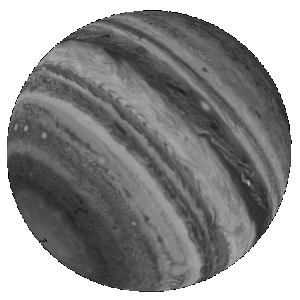
\includegraphics[width=0.25\textwidth]{img/sph_def.png}} \hspace{.0\textwidth} 
\caption{Porównanie wyglądu planet i ilości wierzchołków}
\end{figure}

\paragraph{}

U podstaw pomysłu na zredukowanie ilości wierzchołków do czterech leży spostrzeżenie że tak naprawdę kula wygląda z każdej strony dokładnie tak samo. Ponieważ siatki trójkątów nie korzystają z tego faktu, i dość kiepsko radzą sobie z płynnymi powierzchniami, kula staje się dla nich bardzo trudnym obiektem. Jeśli by natomiast generować geometrię kuli w inny sposób, dało by się bardzo wiele zaoszczędzić.

\paragraph{}

Jak już ustaliliśmy, dla wygenerowania finalnego obrazu potrzebne nam są przede wszystkim pozycja i normalna powierzchni w danym pikselu. Reszta danych zawartych w buforze geometrii jest stała dla planety i można ją otrzymać w oczywisty sposób. Jedynym wyjątkiem jest teksturowanie, które jednak zostanie opisane w rozdziale \hyperref[sub:nakladanie tekstur]{\ref{sub:nakladanie tekstur}}. Pozycje powierzchni planety jesteśmy w stanie łatwo obliczyć posiadając pozycję środka planety, oraz normalną planety w danym pikselu, według wzoru:

\begin{equation} \label{eq:pos}
pozycja = normalna \cdot promien + srodek\_planety
\end{equation}

Potrzebujemy więc otrzymać jedynie normalną w danym pikselu i będziemy mogli skonstruować cały bufor geometrii. Pomysł na wygenerowanie geometrii kuli, polega na stworzeniu dwuwymiarowej mapy normalnych kuli, następnie wstawieniu jej w odpowiednie miejsce w buforze geometrii. Najlepszym sposobem na stworzenie takiego bufora z mapami normalnych, jest wyświetlenie kwadratów w miejscach planet, o boku długości średnic planet, oraz oteksturowanie ich mapą normalnych. W ten sposób to OpenGL będzie odpowiedzialny za skalowanie, clipping, oraz wyświetlenie planety w odpowiednim miejscu. Teksturowanie również należy do banalnych czynności wykonywanych przez bibliotekę graficzną. Fragment shader będzie potrzebny do policzenia pozycji powierzchni planety z normalnej, według wzoru \hyperref[eq:pos]{\ref{eq:pos}}.

\paragraph{}

\begin{figure}
\centering
\label{fig:proj}
	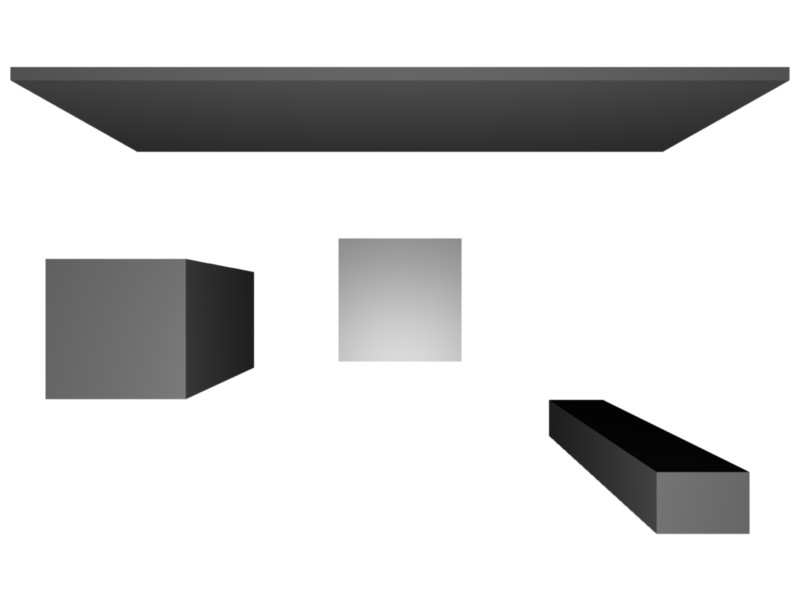
\includegraphics[width=0.5\textwidth]{img/proj_rend.jpg}
\caption{Rzut perspektywiczny sześcianów}
\end{figure}

Powyższy algorytm byłby prawdziwy, gdyby zastosowany został rzut ortogonalny. Ponieważ jednak w symulacjach o wiele bardziej naturalny jest rzut perspektywiczny, należy przystosować do niego powyższy algorytm. W rzucie perspektywicznym, jak pokazane na obrazku \hyperref[fig:proj]{\ref{fig:proj}}, w zależności od pozycji obiektu względem kamery, może być widoczny z różnych stron. Dodatkowo obiekty znajdujące się na brzegu kamery ulegają zniekształceniu z powodu dystorsji. Aby realistycznie oddać rzut perspektywiczny należy uwzględnić te dwa efekty. Dystorsję obiektywu można uzyskać poprzez obrócenie kwadratów na które nakładana jest mapa normalnych, tak aby zwrócone były w stronę kamery. Oznacza to że normalna powierzchni dowolnego kwadratu, jest równoległa do prostej łączącej środek kwadratu (pozycję planety) z pozycją kamery. W ten sposób kwadraty te zostaną przekształcone macierzą projekcji, tak że będą w miarę realistycznie oddawać zniekształcenia obiektywu. Drugim problemem są źle obrócone normalne. Jedynym wyjściem jest dla każdej normalnej, obrócenie jej tak aby była poprawna. Obrót ten musi zostać wykonany o taki sam kąt, o jaki obrócony został kwadrat danej planety. Ponieważ obydwa te obroty są dokładnie takie same, wystarczy dla każdej planety skonstruować jedną macierz rotacji i przemnożyć przez nią zarówno normalne, jak i wektory tworzące kwadrat planety.

% Wstawić wynik renderowania normalny? Wymaga to niestety koloru:/

\paragraph{}

Dodatkowo do mapy normalnych należy dodać informację o przezroczystości danego obszaru. Dzięki temu, rogi kwadratu wyświetlającego planetę, będą mogły być przezroczyste. Planeta będzie miała więc przezroczystość ustawioną na 1.0 lub 0.0. Podczas renderowania, wszystkie piksele których przezroczystość jest mniejsza od ustalonej wartości (np. 0.1) nie zostaną wyświetlone. Sprawi to że wyświetlane kwadraty będą wyglądały jak koła, a po dodaniu oświetlenia i tekstur, staną się ładnymi kulami.

\subsection{Obliczanie oświetlenia}\label{sub:obliczanie oświetlenia}
\paragraph{}

Obliczanie oświetlenia na podstawie buforów ekranów nie stanowi problemu. W programie zastosowane jest model oświetlenia Phonga, natomiast obliczenia prowadzone są dla każdego piksela oddzielnie. Dodatkowo w celach optymalizacyjnych, nie jest liczone światło odbite (specular), ponieważ planety mają powierzchnię chropowatą, więc i tak oświetlenie to by miało znikomy wpływ na efekt końcowy, natomiast jest dość kosztowne obliczeniowo.

\paragraph{}

W celu optymalizacji, dodatkowo do każdej gwiazdy (źródła światła) przypisany jest jej zakres świecenia. Dzięki temu oświetlenie z gwiazd, które nie oświetlają planet odległych od siebie, nie jest obliczane. W przypadku gwiazd nie jest to tak znaczna optymalizacja jak w przypadku bardzo słabych świateł, jak na przykład lampki choinkowe, jednak sprawdza się przy kilku odległych od siebie galaktykach.

\subsection{Nakładanie tekstur}\label{sub:nakladanie tekstur}
\paragraph{}

Skomplikowaniu ze względu na użycie deferred renderingu uległo niestety nakładanie tekstur na planety. Tekstura, tak samo jak wspomniana wcześniej mapa normalnych, jest nakładana na kulę w zależności od koordynat na osiach OX i OY. Jednak w odróżnieniu od mapy normalnych, tekstura zależy od obrotu kamery względem planety, i z każdej strony wygląda inaczej. Pojawiły się więc dwa problemy. Obracanie koordynat tekstury, tak aby widz miał wrażenie że planeta faktycznie się obraca, oraz mapowanie koordynat kwadratu reprezentującego planetę, na koordynaty tekstury planety.

\paragraph{}

Pierwszy problem został rozwiązany poprzez przekazywanie obrotu kamery do silnika graficznego, poprzez przekazanie macierzy obrotu kamery. Następnie uzyskane koordynaty kuli, są przemnażane przez tą macierz. W ten sposób otrzymywany jest bezwzględna pozycja kuli, na którą patrzy aktualnie kamera.

\paragraph{}

Drugim problemem jest mapowanie tekstury na kulę, tak aby z koordynat kuli 3D, uzyskać koordynaty na teksturze 2D. W standardowym podejściu, stosuje się siatki tekstury, natomiast każdy trójkąt jest interpolowany na płaszczyźnie. W naszym podejściu nie ma trójkątów, trzeba więc było uzyskać ciągły sposób mapowania, bez żadnych siatek. Z pomocą przyszła kartografia, która zna liczne sposoby mapowania płaszczyzny na kulę i z powrotem. Najlepsze okazały się metody mapowania o stałej powierzchni. Oznacza to że parametrem który nie ulega zniekształceniu ze względu na położenie na kuli, jest powierzchnia. Dzięki temu po mapowaniu tekstury na kulę, zniekształcenia są najmniejsze. Najtańszą obliczeniowo z tych metod okazała się metoda sinusoidalna, która wymaga policzenia jedynie jednego sinusa.

\subsection{Atmosfery}\label{sub:atmosfery}
\paragraph{}

